\documentclass[11pt,a4paper,oneside]{report}             % Single-side
%\documentclass[11pt,a4paper,twoside,openright]{report}  % Duplex

%\PassOptionsToPackage{chapternumber=Huordinal}{magyar.ldf}
\usepackage{t1enc}
\usepackage[utf8]{inputenc}
\usepackage{amsmath}
\usepackage{amssymb}
\usepackage{enumerate}
\usepackage[thmmarks]{ntheorem}
\usepackage{graphics}
\usepackage{epsfig}
\usepackage{listings}
\usepackage{color}
%\usepackage{fancyhdr}
\usepackage{lastpage}
\usepackage{anysize}
\usepackage[magyar]{babel}
\usepackage{sectsty}
\usepackage{setspace}  % Ettol a tablazatok, abrak, labjegyzetek maradnak 1-es sorkozzel!
\usepackage[hang]{caption}
\usepackage[unicode]{hyperref}

%--------------------------------------------------------------------------------------
% Main variables
%--------------------------------------------------------------------------------------
\newcommand{\vikszerzo}{Hajnal Máté}
\newcommand{\vikkonzulens}{Dr. Imre Sándor}
\newcommand{\vikcim}{Kvantumkommunikációs közösségi könyv: QOS}
\newcommand{\viktanszek}{Hálózati Rendszerek és Szolgáltatások Tankszék}
\newcommand{\vikdoktipus}{Kvantuminformációs Rendszerek - Házi Feladat}
\newcommand{\vikdepartmentr}{Hajnal Máté}

%--------------------------------------------------------------------------------------
% Page layout setup
%--------------------------------------------------------------------------------------
% we need to redefine the pagestyle plain
% another possibility is to use the body of this command without \fancypagestyle
% and use \pagestyle{fancy} but in that case the special pages
% (like the ToC, the References, and the Chapter pages)remain in plane style

\pagestyle{plain}
%\setlength{\parindent}{0pt} % áttekinthetõbb, angol nyelvû dokumentumokban jellemzõ
%\setlength{\parskip}{8pt plus 3pt minus 3pt} % áttekinthetõbb, angol nyelvû dokumentumokban jellemzõ
\setlength{\parindent}{12pt} % magyar nyelvû dokumentumokban jellemzõ
\setlength{\parskip}{0pt}    % magyar nyelvû dokumentumokban jellemzõ

\marginsize{35mm}{25mm}{15mm}{15mm} % anysize package
\setcounter{secnumdepth}{0}
\sectionfont{\large\upshape\bfseries}
\setcounter{secnumdepth}{2}
\singlespacing
\frenchspacing

%--------------------------------------------------------------------------------------
%	Setup hyperref package
%--------------------------------------------------------------------------------------
\hypersetup{
%    unicode=false,             % non-Latin characters in Acrobat’s bookmarks
    pdftitle={\vikcim},        % title
    pdfauthor={\vikszerzo},    % author
    pdfsubject={\vikdoktipus}, % subject of the document
    pdfcreator={\vikszerzo},   % creator of the document
    pdfproducer={Producer},    % producer of the document
    pdfkeywords={keywords},    % list of keywords
    pdfnewwindow=true,         % links in new window
    colorlinks=true,           % false: boxed links; true: colored links
    linkcolor=black,           % color of internal links
    citecolor=black,           % color of links to bibliography
    filecolor=black,           % color of file links
    urlcolor=black             % color of external links
}

%--------------------------------------------------------------------------------------
% Set up listings
%--------------------------------------------------------------------------------------
\lstset{
	basicstyle=\scriptsize\ttfamily, 				% print whole listing small
	keywordstyle=\color{black}\bfseries\underbar, 	% underlined bold black keywords
	identifierstyle=, 								% nothing happens
	commentstyle=\color{white}, 					% white comments
	stringstyle=\scriptsize\sffamily, 				% typewriter type for strings
	showstringspaces=false,     					% no special string spaces
	aboveskip=3pt,
	belowskip=3pt,
	columns=fixed,
	backgroundcolor=\color{lightgray},
} 		
\def\lstlistingname{lista}	

%--------------------------------------------------------------------------------------
%	Some new commands and declarations
%--------------------------------------------------------------------------------------
\newcommand{\code}[1]{{\upshape\ttfamily\scriptsize #1}}

% define references
\newcommand{\figref}[1]{\ref{fig:#1}.}
\renewcommand{\eqref}[1]{(\ref{eq:#1})}
\newcommand{\listref}[1]{\ref{listing:#1}.}
\newcommand{\sectref}[1]{\ref{sect:#1}}
\newcommand{\tabref}[1]{\ref{tab:#1}.}

\DeclareMathOperator*{\argmax}{arg\,max}
%\DeclareMathOperator*[1]{\floor}{arg\,max}
\DeclareMathOperator{\sign}{sgn}
\DeclareMathOperator{\rot}{rot}
\definecolor{lightgray}{rgb}{0.95,0.95,0.95}

\author{\vikszerzo}
\title{\viktitle}
\includeonly{
	guideline,%
	project,%
	titlepage,%
	declaration,%
	abstract,%
	introduction,%
	chapter1,%
	chapter2,%
	chapter3,%
	chapter4,%
	conclusion,%
	acknowledgement,%
	appendices,%
}
%--------------------------------------------------------------------------------------
%	Setup captions
%--------------------------------------------------------------------------------------
\captionsetup[figure]{
%labelsep=none,
%font={footnotesize,it},
%justification=justified,
width=.75\textwidth,
aboveskip=10pt}

\renewcommand{\captionlabelfont}{\small\bf}
\renewcommand{\captionfont}{\footnotesize\it}

%--------------------------------------------------------------------------------------
% Table of contents and the main text
%--------------------------------------------------------------------------------------
\begin{document}
\pagenumbering{Alph}
\onehalfspacing
%--------------------------------------------------------------------------------------
%	The title page
%--------------------------------------------------------------------------------------
\begin{titlepage}
\begin{center}
\includegraphics[width=150mm,keepaspectratio]{figures/eiffel_tower.png}\\
\vspace{0.3cm}
\textbf{Budapesti Mûszaki és Gazdaságtudományi Egyetem}\\
\textmd{Villamosmérnöki és Informatikai Kar}\\
\textmd{\viktanszek}\\[5cm]

\vspace{0.4cm}
{\huge \bfseries \vikcim}\\[0.8cm]
\vspace{0.5cm}
\textsc{\Large \vikdoktipus}\\[4cm]

\begin{tabular}{cc}
 \makebox[7cm]{\emph{Készítette}} & \makebox[7cm]{\emph{Konzulens}} \\
 \makebox[7cm]{\vikszerzo} & \makebox[7cm]{\vikkonzulens}
\end{tabular}

\vfill
{\large \today}
\end{center}
\end{titlepage}



\pagenumbering{arabic}
%----------------------------------------------------------------------------
% Abstract in hungarian
%----------------------------------------------------------------------------
\chapter*{Összefoglaló}\addcontentsline{toc}{chapter}{Összefoglaló}

\hspace{2mm} Ez a dokumentum a Hálózati Rendszerek és Szolgáltatások tanszék Kvantuminformatika és kommunikáció nevezetű tantárgy házi feladatának teljesítésére készült.
A házi feladat egy a kvantumkommunikációs közösségi könyv számára írt fejezet megalkotása volt.
A lehetséges témák közül a QOS-t (Quantum Operating Systems) azaz a Kvantum Operációs Rendszer bemutatását választottam.

\indent Hogyha a kvantum-komputerek mindennapossá válnak világunkban, akkor az operációs rendszernek is tudnia kell biztosítani az újszerű absztrakciót ennek a bizar új hardwer erejének megszelidítéséhez.
Ezen dokumentumban végigvesszük a problémákat, ami ebből a meglehetősen nagy feladatból fakad.
Ezen kívül demonstráljuk, hogy ezek a gépek milyen meglepő sebességnövekedést okoznak sok mindennapos rendszerfeladat ellátására, mint a unit-testing vagy a CPU ütemezés.
Magának az alkotásnak az alapját Henry Corrigan Gibbs, David J. Wu, és Dan Boneh Stanfordi kutatók 2017-ben megjelent Quntum Operating Systems című cikkük jelenti.
\tableofcontents\vfill
%----------------------------------------------------------------------------
\chapter*{Bevezető}\addcontentsline{toc}{chapter}{Bevezetõ}
%----------------------------------------------------------------------------

\hspace{2mm} Az elmúlt néhány évben hatalmas fejlődés volt a nem-triviális kvantumszámítógépek készítése terén.
Rengeteg start-up dolgozik a technológia üzleti alapokra helyezésével, a NIST standardizálja az új "post-quantum" titkostítási rendszerét, és ipari nagyóriások, mint a Google és a Microsoft, tesznek lépéseket manapság, hogy megvédjék rendszereiket a jövőben lehetséges rosszindulatú kvantumtámadásoktól.
Ezek a széleskörben alkalmazható kvantumszámítógépek már a mi életünk alatt is megszülethetnek.

\indent Az első elektromos számítógépek - a Mark I, Clossus, és ENIAC - drágák, nehezen használhatóak és lassú gépek voltak, elsősorban csak a kormánynak dolgozó kódfeltörőknek és a hadifegyver-készítőknek voltak csak hasznára.
Hasonlóan ezekhez a gépekhez az első kvantumszámítógépek is drágák, lassúak lesznek és alkalmazásuk csak a hagyományos titkosítási rendszerek feltörésére, mint az RSA, valamint a fizaki szimulációk futtatására fog kiterjedni.

\indent Szerencsére számunkra, az idővel a klasszikus számítógépek hardvere olcsóbbá és gyorsabbá vált, és a modern operációs rendszerek által biztosított hardver-absztrakciók, virtuális memória, és időosztás  a számítógéper könnyebben használhatóvá, biztonságosabbá és gyorsabbá tették a mindennap embere számára.

\indent A kérdés tehát, hogy az új kvantumszámítógépeink milyen architektúrát igényelnek és, hogy a milyen operációs rendszer is fog ezeken a gépeken futni?
Ebben a dokumentumban felfedezhetjük a \textit{kvantum operációs rendszer} lehetőségeit, kérdéseit azokkal a részleges válaszokkal, amik egy ilyen új típusú operációs rendszer tervezéséhez kellenek.
\begin{itemize}
\item Milyen új absztrakciók szükségesek egy kvantum operációs rendszer programozásához?
\item A kvantum számítógépek ereje, hogyan tudja megnövelni a klasszikus rendszerek teljesítményét?
\item Hogyan nézne ki egy elosztott kvantum számítógép? És milyen új funkcionalitást tud egy ilyen gép biztosítani?
\end{itemize}

\indent Ez a dokumentum szükségesen (és szégyenszerűen) spekulatív:
Még túlságosan korai egy pontos leírást adni egy csak 20, 50 vagy 100 év múlva létező hardverre...
Egyelőre annyit tehetünk, hogy a meglévő kvantumszámlálási modelleket ráillesztjük egy ilyen széleskörű kvantumszámítógépre, hogy elképzeljük milyen lesz majd az, amikor a jövőben megvalósul.

\indent Az olvasó meglehetősen szkeptikusan nézheti most ezt a dokumentumot, mint egy összefoglalója a negatív eredményeknek: a jelenlegi ismereteink szerint, nincs túl sok olyan dolog most, amit a felhasználó egy kvantumszámítógéppel tud csak megcsinálni és egy hagyományos gyors klasszikus számítógéppel nem.
A célünk hát szimplán, hogy tegyünk egy megjegyzést a kvantum számítógépeknél arra a logikus kérdésre, hogy milyen lenne, ha ott lenne mindannyiunk asztalán egy ilyen mágikus kvantumszámítógép?

\indent A dokumentumban három lehetséges architektúrát vázolunk fel, haladva a legkevésbé merésztől a legmerészebb elképzelésig:
Először is a kvantum FPGA-król ejtünk szót, utána a kvantum x86-os számítógépekről, és végül a kvantum elosztott rendszerekről.
Mindegyiknél fogjuk tárgyalni, hogy a gép hogyan kezelné a legalapvetőbb feladatokat, mint a fuzz tesztelés, CPU ütemezés és párhuzamos programozás.
Beszélünk arról is, hogy az egyes architektúrák hogyan felelnek meg a rendszerszintű kihívásoknal.

%----------------------------------------------------------------------------
\chapter{C-RAN koncepció}\label{sect:CranConcept}
%----------------------------------------------------------------------------
\section{Mi is az a C-RAN?}

\hspace{2mm}\cite{RecentCRANProg} \cite{Architecture} \cite{ImplementationIssues} \cite{BenefitsFujitsu} \cite{BenefitsEricsson} \cite{WirelessFull}  \cite{FutureCarrier} \cite{ImplementingGPP} \cite{NokiaSingle} \cite{TechOverview}   Az amerikai származású gépész mérnök Henry Gantt-tól származik a nevét is örző Gannt diagramm forma. Ma már a projektmenedzsment mindennapjait kiséri végig ez a feladatok ütemezését vizuálisan megragadó eszköz. Maga a diagram egy elfektetett oszlopdiagramhoz hasonlít, amelyen követhetjük a projekthez tartozó egyes feladatok elvégzésének egy ütemezését. \cite{GanttChart} Két nagyobb megjelenítendő részből áll, egy a feladatokat listázza, egy pedig a naptárszerű rész mely az elvégzési ütemtervet mutatja. 

\begin{figure}[!ht]
\centering
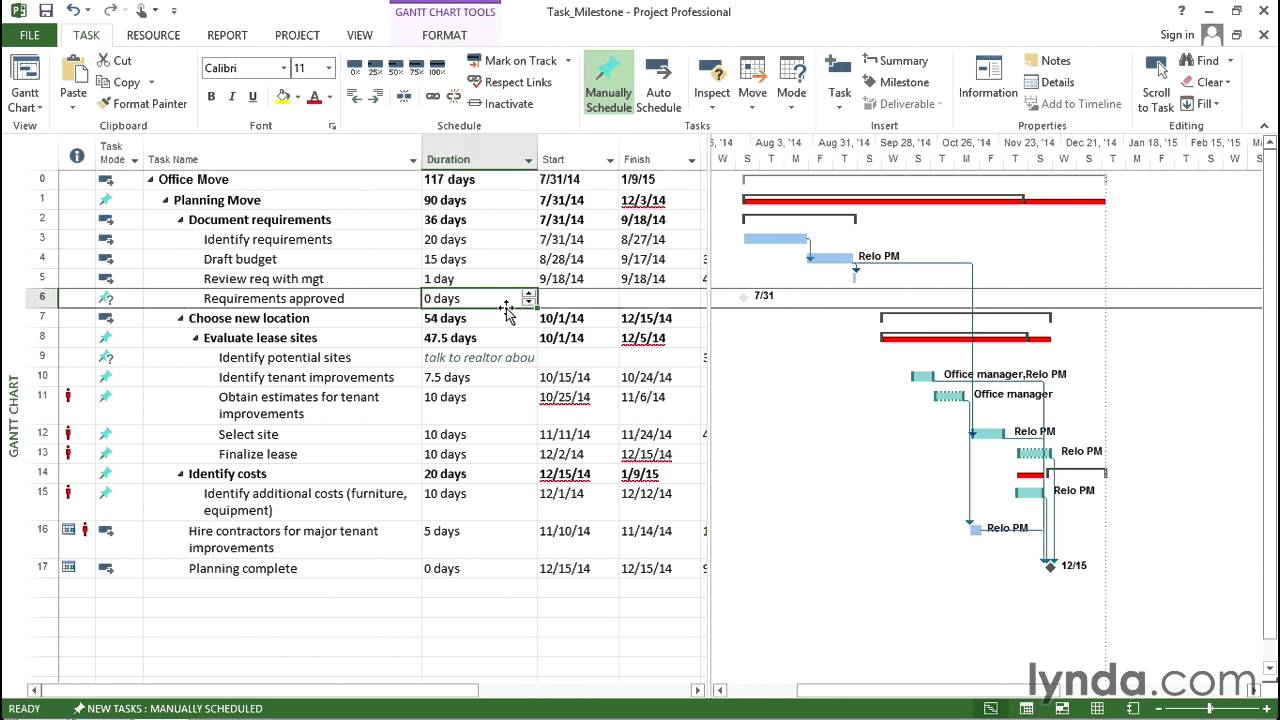
\includegraphics[width=\textwidth, keepaspectratio]{figures/msproject.jpg}
\caption{Microsoft Project 2016 Gantt program kinézete} 
\label{fig:MSProject}
\end{figure} 

A Microsoft Project által megvalósított Gantt vastag kliens alkalmazásra mutat példát a \figref{MSProject}-es ábra. Az ábrán megfigyelhetők a taskok legfontosabb tulajdonságai. Minden tasknál beállíthatjuk, hogy mennyi ideig fog tartani és, hogy milyen függöségei vannak, ezután a task kezdési és végzési idejét az alkalmazás az ütemezés függvényében állítja majd be. Láthatjuk, hogy nem csak feladatok vannak, hanem azoknak egy öszefoglalója, summaryje is melyek alá több feladat tartozhat. Fontos, hogy ez a summary nem egy külön task, hanem azoknak egy gyűjtője, az elvégzési időtartama is az alatta lévő taskok összege. Még érdemes azt is megemlíteni, hogy a program a taskok egymásutániságát nyílakkal is szemlélteti a jobb érthetőség és vizualizáció érdekében. \cite{RecentCRANProg}

A Microsoft Project ellenpontjaként több projekt próbálta vékonykliensen is megvalósítani az alkalmazást egy webes applikáció keretében, ilyen például a GanttPro, melyben a Microsoft Project legtöbb funkciója implementálásra került. A programba a \figref{GanttPro} ábra nyújt betekintést, feladatom a félév során egy ehhez hasonló alkalmazás alapjainak lefektetése volt.\cite{GanttPro}

\begin{figure}[!ht]
\centering
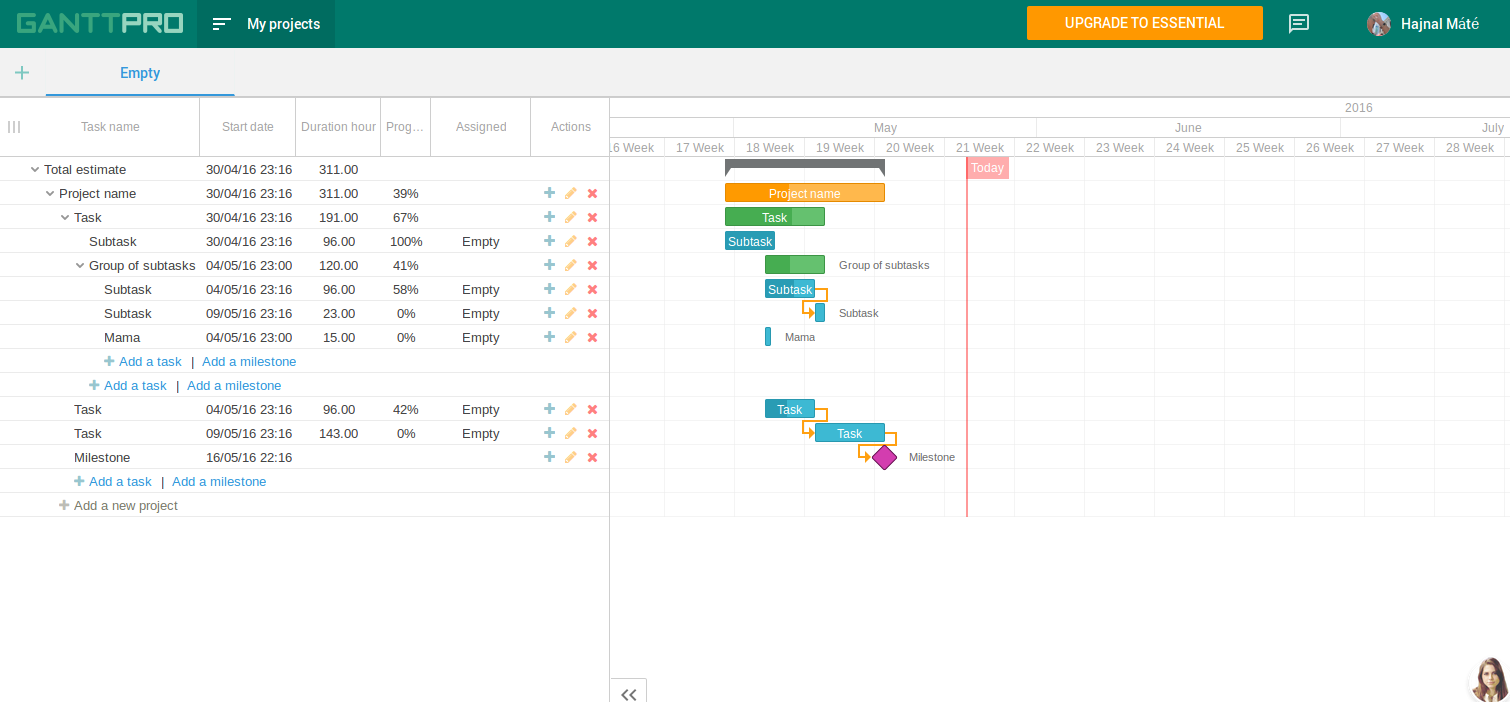
\includegraphics[width=\textwidth, keepaspectratio]{figures/ganntpro.png}
\caption{A GanttPro webes alkalmazás} 
\label{fig:GanttPro}
\end{figure} 

%----------------------------------------------------------------------------
\section{C-RAN Tulajdonságai}
\hspace{2mm} \indent Az irodalomkutatás során az első algoritmus amibe belebotlottam a Kritikus út módszer (Critical Path Method CPM). Maga a Gantt diagram inkább a megjelenítésre fókuszál, a benne lefutó algoritmusokról semmit nem mond, így ezek után az algoritmusok után kellett keresnem a félévben.  Fontos leszögeznem, hogy nincs jelenleg nem NP-nehéz tökéletes megoldása a feladatnak, így a jelenleg legelterjedtebb megoldások közül választottam. A CPM egy ilyen megoldás, mely ha előre ismerjük a feladatok végrehajtási idejét, azok erődorrásait és függőségeit, akkor segít kiszámolni a lehetséges kezdési és befejezési időpontokat. \cite{CPM}

\begin{figure}[!ht]
\centering
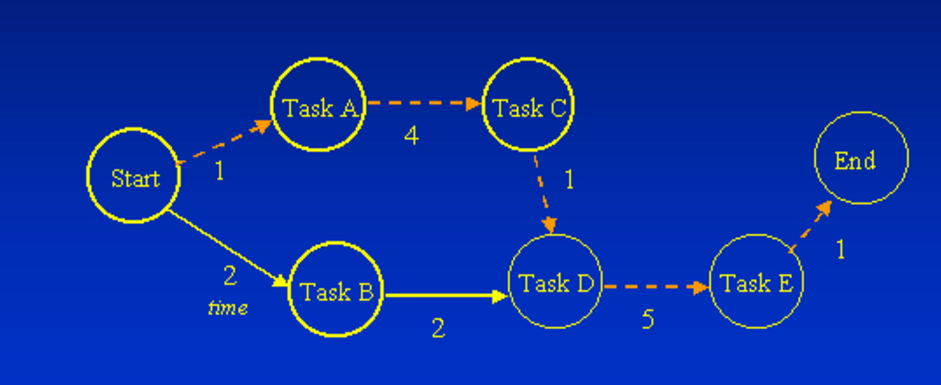
\includegraphics[width=\textwidth, keepaspectratio]{figures/cpm.png}
\caption{A Kritikus út módszerre példa} 
\label{fig:CPM}
\end{figure} 

A \figref{CPM}-es ábrán szemlélhetjük az algoritmus futását. A Start pontból indulunk és a Finish pontba szeretnénk eljutni. Az algoritmus először kiszámítja minden lehetséges útvonalra az úthosszt (ez 11 és 10), ami egy egszerű gráf algoritmust jelent, majd végül a leghosszabb útat választja, ez lesz a kritikus útvonal. Könnyen végig gondolható, hogy azért van ez így, mert a feladatok szempontjából ez az útvonal jelöli a legszűkebb keresztmetszetet, hiszen ennél hamarabb nem tudunk végezni a projekttel.

%----------------------------------------------------------------------------
\section{C-RAN Kihívásai}
\hspace{2mm}  \indent CPM-mel megtaláltuk a projektünk szempontjából legkritikusabb utat, így a végrehajtást ennek az útvonalnak a végigjárásával kell kezdenünk. Viszont a CPM  a projektben lévő többi feladat elvégzéséről nem mond semmit. Ehhez egy másik algoritmust találtam a Least Slack Time scheduling algoritmusát, azonbelül is a First verziót, mely magyarul úgy hangozhat, hogy "Legkisebb tartalékú először" algoritmus.\cite{LST} Az algoritmus lényege, hogy minden feladatnak ad egy prioritást az alapján, hogy mennyire "halogatható" (slack time) az adott feladat. A halogatási időhöz ki kell számolni minden feladatra a legkorábbi kezdési időpontot és a legkésőbbi végzési időpontot, a kettő különbsége a slack time. Ebből az előbbi a CPM algoritmusából már adódik, az utóbbit pedig úgy definiálhatjuk, mint az az időpont, amikor a feladatot legkésőbb végre kell hajtani, hogy ne legyen még csúszás a projektben. Ennek megkapásához egy újabb CPM algoritmust kell futtani úgy, hogy megfordítjuk a futás irányát, azaz a függőségeket és a kezdési időpontnak beállítjuk az utolsó feladat legkorábbi befejezési időpontját. 
%----------------------------------------------------------------------------
\chapter{Programozás házi feladat}\label{sect:ProgHF}
%----------------------------------------------------------------------------

%----------------------------------------------------------------------------
\section{Feladat}
%----------------------------------------------------------------------------

\textit{Egy étteremben a pincérek által felvett rendeléseket egy szekvenciális input fájlban tartják nyilván az ételek neve, azon belül a rendelések időpontja szerint rendezett formában. Feltehetjük, hogy a fájl nem üres. A tárolt adatok: a rendelt étel neve, a rendelés időpontja, rendelt adagok száma, egy adag ára. Melyik étel hozta az étteremnek a legtöbb bevételt (összesített darab*egységár)?}\\

%----------------------------------------------------------------------------
\section{Specifikáció}
%----------------------------------------------------------------------------
A feladat állapottere többféleképpen felírható
% A feladat állapottere
\begin{flalign*}
	A=(f:Infile(&\mathbb{K}),~cout:Outfile(\mathbb{K}))\\
	A=(f:Infile(&Sor),~cout:Outfile(Sor))\\
	A=(f:Infile(&Rendeles), cout:String)\\
	&Rendeles=\textbf{rec}(nev:String, ido:\mathbb{N}, adag:\mathbb{N}, ar:\mathbb{N})\\
\end{flalign*}
Számunkra a legideálisabb már egy olyan felsorolón dolgozni, ami rendelés nevű rekordokat dolgozni, melyek a rendelések nevét és hozzájuk tartozó bevételeket tartalmazzák. Erre a felsorolóra kell nekünk egy maximum keresést írni.\\
% Összegzés, összefűzés
A maximumkeresés:
\begin{flalign*}
	&A=(t:Enor(Rendeles),~cout:String,~max:\mathbb{N},~elem:Rendeles)\\
	&\hspace{25mm}Rendeles=\textbf{rec}(nev:String, bevetel:\mathbb{N})\\
	&Ef=(t=t'~\wedge~|t'|>0~\wedge~t.azon\uparrow)\\
	&Uf=((max,~elem)=\max_{e\in t'}{(e.bevetel)}~\wedge~cout=elem.nev)\\
\end{flalign*}

%----------------------------------------------------------------------------
\section{Absztrakt program}
%----------------------------------------------------------------------------
\begin{center}
\begin{tabular}{|lll|}
	\hline
	\multicolumn{3}{|c|}{\textbf{Maximum~keresés}}\\
	\hline
	t & $\sim$ & \textit{Rendelések bevételeivel való felsorolója}\\
	+,0 & $\sim$~ & \textit{+,0}\\
	f(e) & $\sim$ & \textit{e.bevetel}\\
	\hline
\end{tabular}
\end{center}

\noindent\hfill
	\begin{stuki}[12cm]
		\stm{t.First()}
		\stm{max,~elem:=t.Current().bevetel,~t.Current()}
		\stm{t.Next()}
		\begin{WHILE}{4}{\stm{\lnot t.End()}}
			\begin{IF}[70]{2}{\stm{t.Current().bevetel>max}}
				\stm{max,~elem:=t.Current().bevetel,~t.Current()}
			\ELSE
				\stm{SKIP}
			\end{IF}
			\stm{t.Next()}
		\end{WHILE}
		\stm{cout:=elem.nev}
	\end{stuki}
\vspace{5mm}
\textbf{Rendelések bevételeivel való felsorolója:}
\vspace{5mm}\\
	\begin{tabular}{|l|l|}
		\hline
		\textit{enor(Rendeles)}& \textit{First(),Next(),Current(),End()}\\
		\hline
		\textit{f:Infile(nev:String,ido:$\mathbb{N}$,adag:$\mathbb{N}$,ar:$\mathbb{N}$) }& \textit{First()$\sim$ st, $akt_f$, f:read;Next()}\\
		\textit{st:Status} & \textit{Next()$\sim$ lsd.külön}\\
		\textit{elso:String} & \textit{Current()$\sim$ akt}\\
		\textit{akt:Rendeles} & \textit{End() $\sim$ st=abnorm}\\
		\textit{$akt_f$:rec(nev:String,ido:$\mathbb{N}$,adag:$\mathbb{N}$,ar:$\mathbb{N}$)} & \\
		\hline
	\end{tabular}
\vspace{5mm}\\
\indent A First művelettel beolvastunk a szekvenciális input fájlunkból egy rendelés elemet, melyet az $akt_f$ rekordban tárolunk. A beolvasás sikerességét a státusz jelzés jelzi nekünk.\\
\indent A Next művelet több feladatot, kell ellásson. Addig kell olvasson a szekvenciális input fájlból, amíg a rendelés nevek megegyeznek, vagy véget nem ér a fájl. Ehhez először egy elso nevű változóban eltároljuk az aktuális rendelés nevét, továbbá ehhez hasonlóan egy akt nevű változóban eltároljuk a szükséges rendelés paramétereket, (név és bevétel=adag*ár). Az összegzést, úgy valósítjuk meg, hogy az $akt_f$-be beolvasott input fájl értékek segítségével (az adag*ár értékekkel) az aktuális felsoroló elem $akt$ bevétel nevű változóját növelgetjük. A ciklus akkor marad abba, ha a beolvasás nem sikerült, vagy új rendelésünk van.
\begin{flalign*}	
	&A^{Next}=(f:Infile(nev:String,ido:\mathbb{N},adag:\mathbb{N},ar:\mathbb{N}),elso:String,st:Status,\\
	&\hspace{30mm}act_f:rec(nev:String,ido:\mathbb{N},adag:\mathbb{N},ar:\mathbb{N}),akt:Rendeles)\\
	&Ef^{Next}=(f=f^1~\wedge~st=st^1~\wedge~akt_f=akt_f^1)\\
	&Uf^{Next}=((st=norm\rightarrow elso=akt_f^1.nev\\
	&\hspace{30mm}\wedge~akt.bevetel^2=0)~\wedge~\\
	&(st^2,{akt_f}^2,f^2)=((akt.nev,akt.bevetel)=\sum\limits_{akt_f\in {akt_f}^1,f^1}^{elso=akt_f.nev \wedge st=norm}{(akt_f.nev,} \\
	&\hspace{10mm}akt.bevetel+akt_f.adag*akt_f.ar)\\
\end{flalign*}

\begin{center}
\begin{tabular}{|lll|}
	\hline
	\multicolumn{3}{|c|}{\textbf{Összegzés}}\\
	\hline
	+,0 & $\sim$~ & \textit{+,0}\\
	f(e) & $\sim$ & $akt.bevetel:(akt_f.adag*akt_f.ar)$ \\
	\hline
\end{tabular}
\end{center}

\noindent\hfill
\begin{stuki}[12cm]
	\begin{IF}[70]{2}{\stm{st=norm}}
		\stm{elso,akt.nev,akt.bevetel=\\
		akt_f.nev,0}
	\ELSE
		\stm{SKIP}
	\end{IF}
	\begin{WHILE}{2}{\stm{elso=akt_f.nev \wedge st=norm}}		
		\stm{akt.nev,akt.bevetel:=akt_f.nev,akt.bevetel+akt_f.adag*akt_f.ar}
		\stm{st,akt_f,f:read}
	\end{WHILE}
\end{stuki}


%----------------------------------------------------------------------------
\section{Implementáció}
%----------------------------------------------------------------------------
Program váz: A program több állományból áll: \texttt{etterem.cpp, enor.h, enor.cpp}
\begin{center}
\begin{tabular} {|l|l|l|}
	\hline
	\textbf{etterem.cpp} & \textbf{enor.h} & \textbf{enor.cpp} \\
	\hline
	\texttt{int main()} & \texttt{struct} $Akt_f$ & \texttt{Enor::Read()} \\
	& \texttt{struct Rendeles} & \texttt{Enor::Enor()} \\
	& \texttt{Enor()} & \texttt{Enor::Next()} \\
	& \texttt{void First()} & \\
	& \texttt{void Next()} & \\
	& \texttt{Rendeles Current()} & \\
	& \texttt{bool End()} & \\
	\hline
\end{tabular}
\end{center}
A függvények kapcsolódási szerkezete:\\
\begin{center}
	\begin{tikzpicture}
		[grow=right, align=center, root/.style={rectangle, draw=black, thick, drop shadow, fill=white, text width=5em, rounded corners, minimum height=2em}, leaf/.style={rectangle, draw=black, thick, drop shadow, fill=orange!40, text width=5em, rounded corners, minimum height=2em}, level distance=5cm];
		\node [root] (main) {\textbf{main()}}
			child {node [leaf] (current) {\textbf{Current()}}}
			child {node [leaf] (end) {\textbf{End()}}}
			child {node [leaf] (next) {\textbf{Next()}}
				child {node [leaf] (readb) {\textbf{Read()}}}
			}
			child {node [leaf] (first) {\textbf{First()}}
				child {node [leaf] (reada) {\textbf{Read()}}}
			}				
			child {node [leaf] (enor) {\textbf{Enor()}}};
	\end{tikzpicture}\vspace{2mm}\\
\end{center}
A felsoroló osztálya:\\
	\begin{mdframed}
		\texttt{
		\begin{tabbing}
		\hspace{1cm}\=\textbf{class} Enor\{ \+\\
		    \hspace{1cm}\=\textbf{private:} \+\\
		        \hspace{1cm}\=std::ifstream f;\+\\
		        Status st;\\
		        Rendeles akt;\\
		        $Akt_f$ $akt_f$;\\
		        std::string elso;\\
		        \textbf{void} Read();\\
			\-\\
		    \textbf{public:}\+\\
		        Enor(const std::string \&str);\\
		        \textbf{void} First() \{Read(); Next();\}\\
		        \textbf{void} Next();\\
		        Rendeles Current() \textbf{const} \{ return akt;\}\\
		        \textbf{bool} End() \textbf{const} \{ return st==abnorm;\}\-\-\\
		\};\-\\
		\end{tabbing}
		}
	\end{mdframed}
\vspace{2mm}
Az osztályon belül az input fájl tartalmát egy streamben tároljuk $(ifstream)$, melyből a beolvasás a $<<$ operátor segítségével történik. Az input fájl neve tetszőleges lehet, esetünkben az \texttt{input.txt} nevet kapta. A Read() függvény tölti fel az operátor segítségével az $akt_f$ struktúra változónkat a megfelelő értékekkel.\\
Az aktuális rendelést az $akt$ változóban tároljuk, melynek típusa szintén egy struktúra, neve Rendeles.\\

%----------------------------------------------------------------------------
\section{Tesztelési terv}
%----------------------------------------------------------------------------
A megoldás során két programozási tételt alkalmaztunk az összegzését és a maximum keresését is. Ebből az összegzés tétele annyiszor történik meg, ahány különböző nevű rendelés van. A tesztesetek tehát két részre bomlanak, a maximum keresés teszteseteire és az összegzés teszteseteire, előbbit az utóbbi minden permutációjára meg kell nézni.\vspace{2mm}\\
A fekete doboz tesztesetei:
\renewcommand{\labelenumi}{\Alph{enumi}.}
\renewcommand{\labelenumii}{\arabic{enumii}.}
\begin{enumerate}
	\item \textbf{Maximum keresés} tesztesetei:\\
		\textbf{intervallum hossza} szerint
		\begin{enumerate}
			\item Üres állomány 
			\item Egyetlen üres sort tartalmazó állomány
			\item Egyetlen rendelés
			\item Több rendelés
		\end{enumerate}
		\textbf{intervallum elejes és vége} szerint
		\begin{enumerate}
			\setcounter{enumii}{4}
			\item Az intervallum elején van
			\item Az intervallum közepén van 
			\item Az intervallum végén van
		\end{enumerate}
	\item \textbf{Összegzés} tesztesetei
		\begin{enumerate}
			\setcounter{enumii}{7}
			\item Egy elemet kell összegezni
			\item Több elemet kell összegezni
		\end{enumerate}
\end{enumerate}\vspace{2mm}
A megoldó programra épülő (fehér doboz) tesztesek:
\renewcommand{\labelenumi}{\arabic{enumi}.}
\begin{enumerate}
	\item Hibás vagy nem létező állománynév megadása.
	\item Nem megfelelően kivitelezett bemeneti állomány -> nem megfelelő eredmény, de a beolvasások megtörténnek.
\end{enumerate}
Mindkét tesztesetet a feladat szerint kizárhatjuk.
%----------------------------------------------------------------------------
\chapter{Helyszín}\label{sect:Place}
%----------------------------------------------------------------------------
\hspace{2mm} Pályázatunk egyik sarokköve, hogy szeretnénk az idei gólyabált egy új helyszínen megrendezni, méghozzá az \textbf{ELTE Lágymányosi Campus Északi tömb}-jében. Tisztában vagyunk vele, hogy révén ez egy új kezdeményezés, így mind a kivitelezés mind a döntésünk indokoltsága több kérdést vet fel. Ezeket a kérdéseket a következő alfejezetekben igyekszünk megválaszolni.\\
\indent Az új helyszín gondolata már az elmúlt években is felmerült és leginkább anyagi okai vannak/voltak annak, hogy a Dürer rendezvényházban (Dürlin) tartottuk a Gólyabálunkat. Ez a lehetőség tudomásunk szerint idén még fenn áll, így ha bármi probléma merül fel az Északi tömbbel a Dürlin, mint mentő opció tökéletes lehetőség. Ettől az opciótól nem is szeretnénk elzárkózni. Erre a helyszínre már az elmúlt években kialakult egy majdnem optimális elrendezés, ettől ebben az esetben nagymértékben nem is térnénk el.\\
\indent Mivel a Dürlin-t jövőre felújítják, így mindenképpen új helyszínt kell majd keresnünk. Úgy gondoltuk, hogy a legjobb megoldás a probléma elé menni. Tavaly Barbiék nagyon sok helyszínt megnéztek, melyek listáját el is kértük tőlük. Szerintünk ezeknek a köröknek az újra járása nem sok eredményhez vezetne, ez az Északi tömb nyújtja az általunk vélt legjobb megoldást.
\begin{wrapfigure}[10]{l}{0.40\textwidth} 
\begin{center}
\includegraphics[width=0.35\textwidth, keepaspectratio]{figures/moulin1.jpg}
\end{center}
\caption{Moulin Rouge} 
\label{fig:Moulin}
\end{wrapfigure}

%----------------------------------------------------------------------------
\section{Eredet}
%----------------------------------------------------------------------------
\indent Az ötlet, hogy az Északi tömbben rendezzük a bálunkat, az idei SOTE-s Karnevál nyomán merült fel bennünk. Az IÖCS által szervezett Nemzetközi Semmelweis Karnevál egy körülbelül 1900 fős rendezvény melyet minden évben megrendeznek, idén április 2-án került rá sor. A Karnevált rendszerint a NET-ben (Nagyváradi Elméleti Tömb) szokták tartani, ám idén felújítások miatt erre nem volt lehetőségük, így jutottak el az Északi tömbhöz, mint helyszín.\\
\indent	Megkerestük a Karnevál egyik főszervezőjét, Klément Emesét (Mesit) a részletekkel kapcsolatban, aki rengeteg kérdésünkre válaszolt és egy nagyon pozitív feedbacket adott a helyről. Mesitől elkérve a hely kontaktját, jutottunk el Garab Emilhez (egarab@gmail.com, 20/925-7422), aki a Lágymányosi épületek rendezvényekkel kapcsolatos felelős személye. Emillel közös beszélgetéseink során igyekeztünk minden részletet megtudni, melyek a megvalósításhoz kellenek, ezekre Ő készségesen válaszolt és még a legutolsó kérdéseinket is tisztázta egy az Északi tömbben való tárlatvezetés alkalmával.

%----------------------------------------------------------------------------
\section{Új helyszín pro-kontra}
%----------------------------------------------------------------------------
\subsection{Ár}
\hspace{2mm} Az első nagy kérdés számunkra a helyszín ára volt. A SOTE-sok összesen bruttó 1,53milllió forintért bérelték a helyszínt. A jelenlegi lovagrendi gazdaságist Barbit megkérdezve, a Dürlin 900 ezer forintba került.  Első látásra mi is elszomorodtunk, de kiderült, hogy a bérlés sok részre diverzifikálható. A Karnevál majd 700 fővel nagyobb rendezvény, mint a miénk, így mi nem igénylünk akkora teret mint ők.\\
\indent A helyszínbérlés náluk négy összetevőből állt, 582 ezer forintért bérelték a Gömb Aulát, 218 ezer forintért a Gömb Aulához tartozó karzatot, 400 ezer forintért a Harmónia termet és 4 nagy tantermet darabonként 72, valamint 5 kicsit darabonként 8 ezer/14 ezer forintért. A helyszínből, ami mindenképpen kell nekünk az a Gömb Aula, a felette lévő karzat és legalább kettő kis terem, így árban kicsit több, mint 800 ezer forintét már tudunk helyszín-ügyileg itt Gólyabált rendezni.  A helyszínt bejárva viszont az optimális (számunkra szerintünk legideálisabb) elrendezést tekintve, 3 nagy tanterem és 3 kicsi tanterem kell (a Harmónia terem semmiképp sem), így a végösszeg kicsit több, mint 1,05 millió forintra jön ki, amely 150 ezer forinttal jelent többet, mint a Dürlin. Mivel a helyszín rengeteg előnnyel jár, ez a plusz költség rengeteg más helyen megtérül (tranzit, gombák, sátrak bérlése jelentős kiesést jelent, plusz Gólyabál busz sem kell), így ez a plusz költség szerintünk belefér. Természetesen hogyha mégsem fér bele módosítjuk majd a terveinket, mindenesetre pályázatunkban ez alapján terveztünk és Emiltől is ezek alapján már kértünk egy előzetes árajánlatot.

\subsection{Kontra}
\hspace{2mm} A helyszín legnagyobb -- és egyetlen -- ellenérve az, hogy mivel az ELTE-n hétköznap tanítás van, így a bált csak szombati napon tudjuk megrendezni. Az ELTE PPK-n már 4 éve gond, hogy szeretnék a bált csütörtök megtartani, mert náluk “mindenki” haza megy már csütörtök este, így a pénteki időpontokba is ódzkodva mentek bele. Továbbá, nem tudhatjuk hány embert veszítünk el a pénteki helyett szombati időpont miatt (a péntek egyszerűen csak ideálisabb a gólyáknak). \\
\begin{wrapfigure}[12]{r}{0.2\textwidth} 
\begin{center}
\includegraphics[width=0.18\textwidth, keepaspectratio]{figures/eiffel2.jpg}
\end{center}
\caption{Eiffel torony} 
\label{fig:Eiffel}
\end{wrapfigure}
\indent Fontos megemlíteni, hogy a szombati időpont a fentebb említettekkel szemben pozitívumokat is rejt magában. Először is a rendezés során rendszeresen probléma volt, hogy péntek reggel sok embernek még ZH-ja volt, így sok rendező nem tudott bevállalni egy reggeli pakolást vagy csütörtök esti utolsó gyűlést. Ez a probléma egy az egyben megszűnne. Rendezői szempontból ideálisabb a szombati időpont. Ehhez még az is hozzájön, hogy már péntek este elkezdhetjük a helyszín berendezését (ezt Emil kiemelte), így erre bőven elég időnk lenne, nem szükséges a feszített tempó. \\
\indent A szombati időpontnak hála lehetne a Gólyabálnak egy íve. Megkérnénk a ClubCeption-t, hogy csináljanak a Gólyabál előtti péntek este 9-től egy Gólyabál váró bulit, rákészülésképpen és ugyanezen az estén tartanánk egy gyűlést a kisfőnökökkel -- PPK-sok is -- az ENT-ben 8-tól, melyen az utolsó kérdéseket is elsimítanánk. Szombaton megtörténne a Gólyabál és vasárnap Kakasban éjfél kispulton várnánk a (jobb esetben :P) kipihent rendezőket. \\
\indent Úgy érezzük, hogy a PPK-sok a fentebbi érveinket végighallgatva meg fogják érteni a problémánkat és bele fognak egyezni a szombati bál gondolatába.



\subsection{Pro} 
\hspace{2mm} Az új helyszínnek rengeteg előnye van, melyeket a teljesség igénye nélkül szeretnénk felsorolni.
\begin{itemize}
	\item  A Dürlin legnagyobb hátránya az, hogy a táncokat nem lehet jól látni, ezért vetítésekkel oldjuk meg a közvetítést. Ez a probléma teljesen megszűnik, hiszen a Gömb Aulát a karzatról tökéletesen beláthatja az egész közönség.
	\item A Gömb Aula akusztikája világhíres. Hogyha középen dobbant valaki azt az Aula túlsó felében is hallani lehet. Ez hihetetlenül meg tudja emelni a koncertek minőségét és a hangulatot.
	\item A Gömb Aula teteje üvegből van. Ez lenne az első VIK-es Gólyabál, ahol a Holdfénykeringő valóban a holdfényben történik. Az egész Gömb Aula világítását egy helyről lehet kezelni, így a lámpák lekapcsolása egyszerűen kivitelezhető.
	\item Az Északi tömb a rakparton helyezkedik el és mellette található egy móló, ahol ki tud kötni a Gólyahajó, melynek utasai egyből a bálhelyszínre tudnának sétálni. Nem lenne szükséges még villamosozni, mint a Dürlinnél.
	\item A bejárat mellett csigalépcsők visznek le a -1-re, ahol a ruhatárazás tökéletesen megoldható. Itt meg kell említenünk, hogy a helyszín biztosít elegendő fogast, így nem kell a NET-ből kölcsön kérnünk.
	\item A három nagy tanteremből kettő egybe nyitható, melyekben a Borozó és a Kajáspult is kényelmesen elfér. A harmadikban pedig elegendő helyet tudunk biztosítani a Parkettnek.
	\item A tantermekben a padok és asztalok mozgathatók, melyeket oda vihetünk ahova szeretnénk, így nem szükséges a Zé épületből padokat kérnünk, az összes pultot meg tudjuk csinálni iskola asztalokból. 
	\item Mivel nem kell a Zé épületből asztalokat kérnünk egy kis tranzit elég a Gólyabál pakoláshoz, nem kell a teherautó. Ez a Gólyabál költségvetésében is jelentős kiesés. Természetesen plusz sörpadokat még kell majd kérnünk más koliktól pl: Martos, de ez csak egy vagy kettő plusz kis-tranzit kört jelent.
	\item A meghívott körök nyitása a Dürlinhez hasonlósan megoldható a helyszínen. (részletek a következő alfejezetben.)
\end{itemize}

%----------------------------------------------------------------------------
\section{Helyszín tervek}
%----------------------------------------------------------------------------
\hspace{2mm} A helyszínt bejárva, végiggondoltuk az események megvalósítását, melyet igyekeztünk vizuális formában is minél jobban megragadni. Az Északi tömbnek három bejárata van, egy a rakpart felől egy a tudósok körútja felől és egy a Déli tömb felől. Ezek közül a Déli tömb felőli a legszélesebb és kényelmesebb, a többit lezáratnánk. Fontos megemlíteni, hogy ezeket a bejáratokat fizikailag nem lehet becsukni, hisz bármelyik egyetemi tanárnak biztosítanunk kell tudni a bejárást még hajnalban is, így ezekbe rendezőket és biztonsági őröket kell majd állítani, akiknek koordinálását a kapus kisfőnökök fogják végezni. 

\subsection{Beengedés:}
\hspace{2mm} A bejárat előtt lenne a beengedés, itt van egy nagyobb területünk a kordonok lerakásához, és a beengedéshez szükséges infrastruktúra kialakításához. Az egész ELTE kampuszon van Wifi lefedettség, aminek eléréséhez csupán Ceasar azonosítóra van szükség, mellyel minden ELTE-s hallgató rendelkezik (Máténak is van), így ez semmiképp sem jelenthet problémát (Emil azt mondta egy közös, a rendezvényhez tartozó azonosítót is kapnánk).
\indent A főbejárat előtt a beengedés után van egy nagyobb füves rész, melyet engedéllyel használhatunk, és maga az engedély sem drága (Emil azt mondta, hogy nem több 15-20 ezer forintnál). Ennek a füves területnek a nagysága elegendő ahhoz, hogy elhelyezzünk rajta egy szigorúan nem leszúrt akár 6*6 méteres sátrat, melyben a WTF kényelmesen elfér. A területhez az engedélyt és egyébként az egész bérléssel kapcsolatban a szerződést Fehér Ágnessel a kampusz igazgatójának segítségével kötnénk meg. Emil azt mondta, hogyha úgy adódik, akkor szívesen bemutat minket neki. Megemlítenénk még, hogy itt a bejárat előtt van lehetőségünk egy dohányzásra kijelölt terület kialakítására is.

\subsection{Biztonsági őrzés \& tűzvédelem}
\hspace{2mm} A kampuszon a biztonsági őrzésért egy külön cég felel a Dussmann Kft, melynek vezetője Pásztor Zsolt (pasztor.zsolt@dussmann.hu, 20/559-3607). A helyszín ragaszkodik hozzá, hogy valamilyen arányban szerepeljen emberük a rendezvényen, ám nem szükségszerűen kell, hogy ők biztosítsák a teljes biztonsági őrzést. Pontosabban is utánajártunk így a dolognak és számukra elég, ha legalább három biztonsági őr lesz jelen tőlük a rendezvényen. Ebbe úgy érezzük, hogy Orbán Balázsék is bele fognak menni, hiszen az előre láthatólag 11 biztonsági őrből a miénk lesz 8 fő, ami kellemes arány. Zsolt felel az épület tűzvédelmi szabályzatának [3] megfelelő betartásáért is, és felajánlotta nekünk, hogy szívesen csinál egy tűzvédelmi tárlatvezetést a rendezőknek. Ezzel a lehetőséggel szeretnénk is élni, úgy véljük a kapu- és lengő főnököknek semmiképp sem árthat egy ilyen előadás. Természetesen csak számukra lenne ez “kötelező” jellegű más kisfőnököknek nem. 

Készítettünk pár tervezetet a belső elrendezésről, de mivel ezek még folyamatosan változhatnak, így csak később tervezzük minden részletében kidolgozni.
\begin{figure}[t]
\centering
\includegraphics[width=0.6\textwidth]{figures/stamps.jpg}
\caption{Bélyegek}
\label{fig:Stamps}
\end{figure}

%----------------------------------------------------------------------------
\chapter{Összefoglalás}\label{sect:Summary}
%----------------------------------------------------------------------------

\hspace{2mm} Elmondhatom, hogy a félév során rengeteget tanultam, megismerkedtem modern webfejlesztési eszközökkel és implementáltam egy kiterjedt osztályhierarchiával rendelkező komolya naptár kezeléssel bíró webes alkalmazást. 
%----------------------------------------------------------------------------
\chapter{Összegzés}\label{sect:conclusion}
%----------------------------------------------------------------------------
\hspace{2mm} Ha a kvantumszámítógépek valóban az utjukon vannak, akkor a rajtuk futó opercáiós rendszernek kulcsfontosságú szerepe lesz, hogy készíthessünk rajtuk konstruktív alkalmazásokat.
Richard Feymann azt mondta a kvantumszámításról, "Ez egy csodálatos probléma, mert nem tűnik túl könnyűnek."

%\listoffigures\addcontentsline{toc}{chapter}{Ábrák jegyzéke}
%\listoftables\addcontentsline{toc}{chapter}{Táblázatok jegyzéke}

\bibliography{mybib}
\addcontentsline{toc}{chapter}{Irodalomjegyzék}
\bibliographystyle{plain}

\label{page:last}
\end{document}
